\documentclass[final]{svjour2}
\usepackage{amsmath}
\usepackage{graphicx}
\usepackage{rotating}
\usepackage{amssymb}
\usepackage{mathptmx}
\usepackage[numbers]{natbib}
\usepackage{float}
\usepackage[section]{placeins}
\usepackage{tabularx}
\usepackage{booktabs}
\usepackage{color}
\usepackage{epstopdf}
\usepackage[table]{xcolor}
\usepackage{threeparttable}
\usepackage{multirow}

\renewcommand{\thefootnote}{\alph{footnote}}

\makeatletter
\journalname{Journal of Low Temperature Physics}
%%%%%%%%%%%%%%%%%%%%%%%%%%%%%% Textclass specific LaTeX commands.
%%%%%%%%%%%%%%%%%%%%%%%%%%%%%% User specified LaTeX commands.
\bibpunct{}{}{,}{s}{}{,}

\begin{document}

\newcommand{\hdblarrow}{H\makebox[0.9ex][l]{$\downdownarrows$}-}
\title{Material Selection for Cryogenic Support Structures}

\author{E. Kramer \and N. Kellaris  \and M. Daal  \and B. Sadoulet \and S. Golwala \and M. Hollister}

\institute{Department of Physics, U.C. Berkeley,\\ Berkeley, CA 94709, USA\\
\email{ekramer@berkeley.edu}}

\date{XX.XX.20XX}

\maketitle

\begin{abstract}

Design specifications for the support structures of low temperature instrumentation often call for low thermal conductivity between temperature stages, high stiffness, and specific load bearing capabilities.  While overall geometric design plays an important role in both overall stiffness and heat conduction between stages, material selection can affect a structure's properties significantly.  In this contribution, we suggest and compare several alternative materials to the current standard materials for building cryogenic support structures.

\keywords{Cryogenic, Low Temperature, Cryogenic Materials, Thermal Conductivity, Material Strength, Young's Modulus, Cryogenic Support, Support Structures, Truss, Structural Materials}

\end{abstract}

\section{Introduction}

Cryogenic support structures are typically engineered to meet three design specifications: low thermal conductance, high strength, and high stiffness. Creating support structures that obtain the lowest thermal conductance between temperature stages while remaining structurally adequate to support forces imposed during operation at low temperature and handling at room temperature is a design optimization problem. The thermal consideration usually results in structures suspended by elements possessing minimized cross-sectional area such as thin plates, webs of yarn, slender rods, or tubes. The application will dictate which parameter, strength or stiffness, imposes the next most limiting design constraint. Focusing on the case of stiffness, we draw attention to the fact that both stiffness and power conducted are proportional to the cross-sectional area, $A$, divided by the length, $l$, of the structure support members.\cite{Hastings1993} As we will explain, this provides a helpful parameterization for the selection of cryogenic support structural materials.

\section{Design Parameters}

The property that is primarily used to describe the stiffness or elasticity of a material is its Young's modulus. Young's modulus is formally defined for tensile stresses, but for isotropic materials one can extend the notion for use with compressive forces. Young's modulus is sometimes called the {\em elastic modulus} or {\em modulus of elasticity}. It is the ratio of the stress along a given axis over the strain along the same axis in the range of values where Hooke's law holds\footnote{Stress ($\sigma$) here is defined as the force applied in the direction normal to a sample's cross section divided by the cross sectional area of the sample (assuming a constant cross sectional area) $\sigma = F/A_{0}$.  Strain ($\epsilon$) is defined as the change in length of the sample in the direction of the applied force over the original length $\epsilon=\Delta L/L_{0}$.}. Young's modulus can sometimes be different for tensile stress (the {\em tensile modulus}) and the compressive stress (the {\em compressive modulus})\footnote{When tensile and compressive moduli are not equal this is due to an asymmetry (e.g. the specimen is a string), or a rapid variation of the modulus which occurs through zero strain, but this is not a discontinuity in the curve. Materials exhibiting this rapid change in modulus around zero stress are called {\em bimodulus} or {\em bilinear} materials.}. In addition, different samples of the same material may have different moduli as a result of their defect characteristics, heat treatments, etc.

\begin{table}[htb]%THERMOPHYSICAL PROPERTIES
\begin{threeparttable}
\rowcolors{3}{gray!20}{white}
\begin{tabular}{lrrrrrr}
\toprule
\textbf{Material} & $\rho$ ($\frac{g}{cm^3}$) & $\nu$ & $\sigma_{t}$ (MPa) & $\sigma_{c}$ (MPa) & TM (GPa) & CM (GPa) \\
\midrule
 POCO AXM-5Q & 1.73 & 0.27 & 48\tnote{U} & 124\tnote{U} & 10.5 & - \\
 TIMET Ti 15-3-3-3 & 4.78 & 0.36 & 766\tnote{Y} & 810\tnote{Y} & 82.0 & 90.0\\
 Stainless 316LN & 7.99 & 0.29 & 690\tnote{Y} & - & 200.0 & - \\
 Vespel SP-1 & 1.43 & 0.41 & 86 & 133\tnote{*} & 2.5\tnote{\dag} & 2.4 \\
 Vespel SCP-5000 & 1.46 & - & 163 & 230\tnote{*} & 4.0 & 9.1 \\
 Vespel SP-22 & 1.65 & - & 52 & 112\tnote{*} & 2.5 & 3.3 \\
 Vespel SCP-5050 & 1.76 & 0.22 & 72 & 172\tnote{*} & 8.9 & 3.0 \\
 Torlon 4301 & 1.46 & - & 113\tnote{U} & 166\tnote{U} & 6.8 & 5.3 \\
 G-10CR & 1.90 & 0.18 & 429\tnote{U} & 374\tnote{U} & 27.9 & 15.0 \\
 Graphlite CF Rod & 1.55 & -  & 2340 & 1900 & 134.0 & 131.0 \\
 Kevlar 49 Fibers & 1.44 & 0.36 & 3000\tnote{U} & - & 112.4 & - \\
 Macor & 2.52 & 0.29 & 90\tnote{U} & 345\tnote{U} & 66.9 & 64.0 \\

 \bottomrule
\end{tabular}
\caption{Some physical and mechanical properties of candidate materials. $\nu$ is the Poisson's ratio for the material, while $\sigma_{t}$ and $\sigma_{c}$ are the tensile and compressive strengths for the material, respectively. Superscripts on strengths refer to: Y - yield strength, U - ultimate strength, * - compressive load at \%10 strain. Unmarked numbers have unknown failure conditions. TM and CM are the tensile and compressive elastic moduli respectively. A blank indicates that the specified property could not be found in the literature for a given material. Data comes largely from manufacturer's literature; where values were missing from manufacturer literature, outside references were used; references as well as relevant notes about the material properties are as follows: POCO AXM-5Q -- $\nu$ from \cite{Swank2009}; Ti 15-3-3-3 -- $\nu$, $\sigma_t$, $\sigma_c$, CM from \cite{Lang2001}\cite{Johnson1996}\cite{Nyakana2005}. All properties were for solution-treated material; SS316LN -- $\nu$ from \cite{Shankar2001}. Other data are from SS316LN data sheet for cold worked material (www.finetubes.com); Vespel -- TM for SP-1 from \cite{Doty1981}. All data were for isostatically formed parts. $\dag$ - Tensile modulus estimated from manufacturer's stress-strain plot; G-10CR -- all data from \cite{Kasen1981}\cite{Markley1985}. Properties taken in the warp direction; Graphlite CFRP -- properties along the fiber axis; Kevlar 49 -- all data are for unfilled fibers; Macor -- $\sigma_t$ and CM from \cite{Markley1985}\cite{websiteMacor}.}
\label{SW}
\end{threeparttable}
\end{table}

Excepting systems where the stresses are known to be mainly of a certain type (compressive, tensile, shear), it is advisable to design a structure using the smaller of the tensile and compressive moduli.  This allows a sufficient factor of safety to prevent premature failure, regardless of the reaction forces in the structure.

It is also important to note the other properties of the material being used.  Ductile materials, such as most metals, tend to fail from shear forces first, while brittle materials like carbon fibers fail from normal forces first.\cite{Dowling2007}  Another aspect of material selection is metallic versus non-metallic supports. Metallic supports can be quite stiff, however they are not ideal for applications requiring electrically isolated stages.  Also, the shape of the thermal conductivity curve plays an important role, as steep thermal conductivity curves create susceptibility to thermal runaways in the cryostat.

\begin{figure}[ht]
\begin{center}
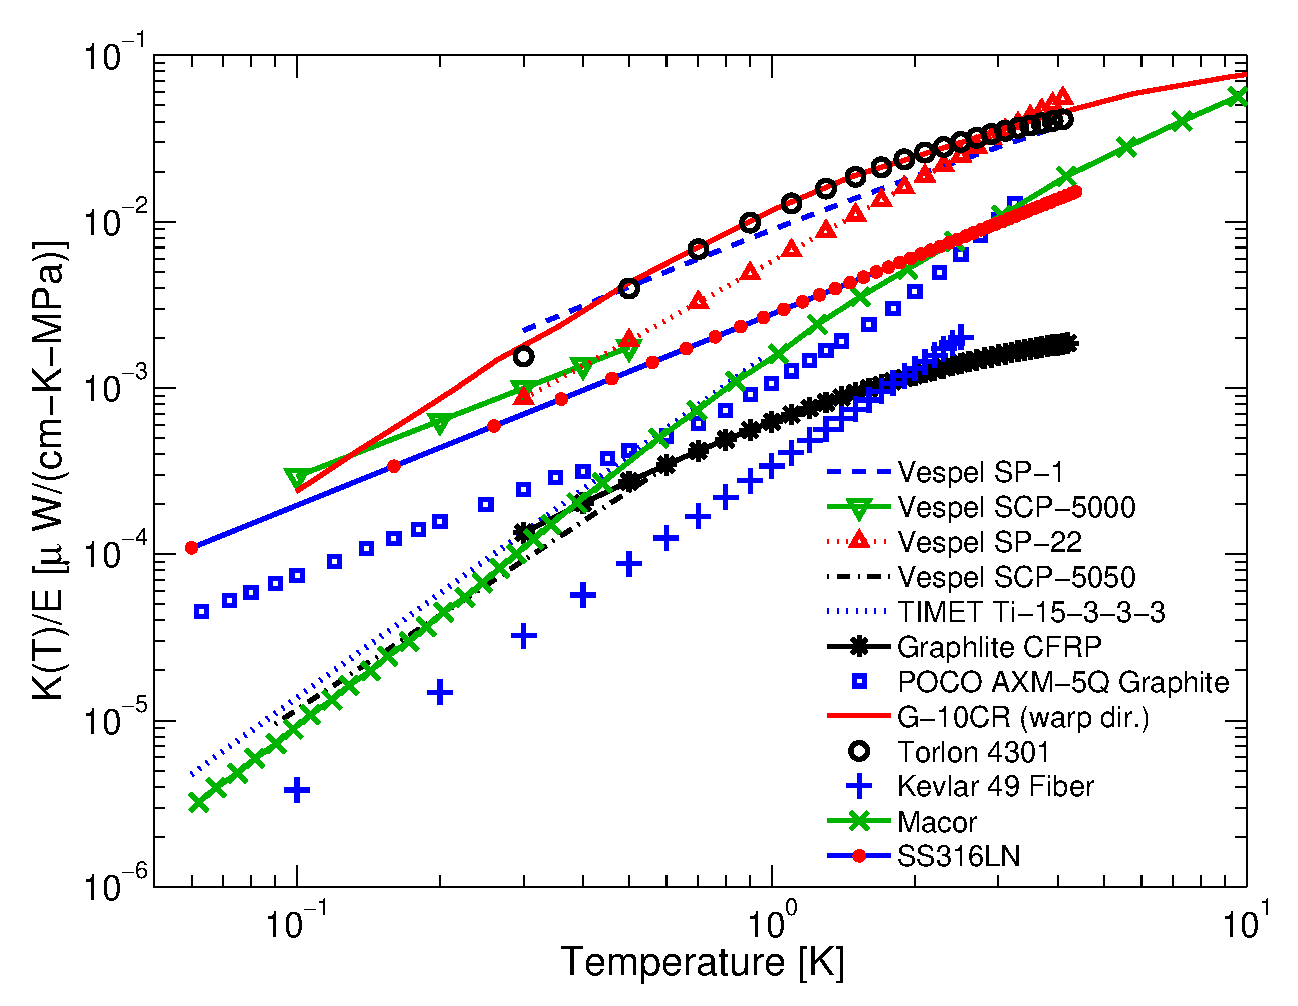
\includegraphics[%
  width=1\linewidth,
  keepaspectratio]{E_norm_support_K.eps}
\end{center}
\caption{A selection of useful materials with their thermal conductivity normalized by their room temperature Young's modulus.  Lower values are desirable as support materials.  Thermal conductivity references: Vespel SP-1, Vespel SP-22, Graphlite CFRP, and Torlon 4301 from Runyan\cite{Runyan2008}; Vespel SCP-5000, Vespel SCP-5050, and Ti 15-3-3-3 (under 20\% cold work after anneal) from Kellaris\cite{Kellaris2013}; AXM-5Q, G-10CR, and Macor from Woodcraft\cite{Woodcraft2009} \cite{Woodcraft2009_2}; Kevlar 49 from Ventura\cite{Ventura2009}; Stainless Steel 316LN from Barucci\cite{Barucci2008}. Young's moduli from Table \ref{SW}.}
\label{Mats}
\end{figure}

Overall, when selecting a material, one must ensure that the final design will be stiff enough to not fail under expected load ranges while keeping its cross section as low as possible to minimize the amount of heat transfer between temperature stages. Since the stiffness of structural elements (such as truss members) and power conducted are both proportional to the cross-sectional area divided by the length \footnote{The common $A/L$ dependence holds for small axial and radial loads. Other loads, such as off axis moments may not have this dependence and may result in structural weaknesses including reduced stiffness.}, $A/l$, we can normalize the thermal conductivity of a material to its Young's modulus to provide a useful metric for comparing materials' performance for use in these structures; high stiffness and low thermal conductance is typically desired, so materials with the smallest thermal conductivity to Young's modulus ratio are ideal\cite{Hastings1993}. Runyan\cite{Runyan2008} et al. use this metric to compare different materials not featured in this contribution. In Fig 1. we present a few newer materials along with familiar standbys that have the desired low thermal conductivity to Young's modulus ratio.

\section{Material Selection}

Materials that tend to be the most useful for creating stiff isolated cryogenic support structures maintain a low thermal conductivity to Young's modulus ratio at low temperatures, relative to other building material types. For the purposes of the Cryogenic Dark Matter Search experiment (with which the authors are involved) design requirements are low thermal conductivity at low temperature and high rigidity at room temperature, because our structure bears no loads in the cryostat during operation but endures stresses during installation and handling. Thus, for this analysis and the data in Fig. \ref{Mats}, we used the room temperature values of Young’s modulus. Many applications and experiments, however, are interested in the low temperature Young's modulus of a material. This data is scarce in the literature, but rather than measure each material of interest, one can develop expectations for the low temperature modulus based on material type (e.g. metals, polymers, ceramics) from the information that does exist in the literature. The results of our literature search can be seen in Table \ref{E_table}. All materials studied in this paper have a Young's modulus which increases with decreasing temperature, thus increasing their stiffness at low temperatures.


\begin{table}[h]

\centering
\begin{threeparttable}
\rowcolors{3}{gray!20}{white}
\begin{tabular}{lrrrrrr}
\toprule
&  \multicolumn{4}{c}{Young's Modulus, E (GPa)} & \multirow{2}{*}{$(E_{300K} - E_{4K})/ E_{300K}$}\\
\textbf{Material} & & \@ \quad\quad 300K & \@ \quad\quad 77K & \@ \quad\quad 4K  \\
\midrule
Ti 6Al-4V & & 110.7 & 114.8 & 123.0 & 11.1\% \\
Ti 5Al-2.5Sn &  & 114 & 120 & 128.0 & 12.3\% \\
SS316 &  & 195.0 & 209.0 & 208.0 & 6.7\% \\
Kapton Film &  & 3.5 & 5.7 & - & $>$ 62.9\% \\
Torlon & & 1.57 & 2.50 & & $>$ 59.2\% \\
G-10CR Warp & & 28.0 & 33.7 & 35.9 & 28.2\% \\
CFRP: T300 fibers  & A  & 132 & 141 & - & $>$ 7.0\% \\
CFRP: T300 fibers & B  & 135 & 137 & - & $>$ 1.5\% \\
CFRP: T700 fibers & & 144 & 166$^+$ & - & $>$ 15.2\% \\
Kevlar 49 fiber & & 98.6 & 172 & - & $>$ 74.5\% \\
Macor & & 64.1 & - & 68.1 & 6.2\% \\


\bottomrule
\end{tabular}
\caption{Young's Modulus as a function of temperature for investigated materials; where no data was found in the literature, proxy materials were used. Modulus values presented may differ from Table \ref{SW}, but are meant to indicate expected variation with temperature, rather than absolute values. Ti 6Al-4V \cite{Meester1975} and Ti 5Al-2.5Sn \cite{Ghisi2007} are similar alloys to Ti 15-3-3-3. SS316: \cite{Reed1983}. Kapton film \cite{Yamaoka1995} is used as a proxy for Vespel products. Torlon \cite{Reed1983}, unspecified grade. G-10CR \cite{Kasen1981}, measured in the Warp direction. CFRP: T300 and T700 fibers \cite{Reed1983}, unidirectional CFRP laminates measured parallel to fiber axis. 'A' and 'B' used low modulus and high modulus resin, respectively. Kevlar 49 fibers \cite{James2012}. Macor \cite{Harrington1980}, elastic modulus determined from measured elastic constants. + indicates Data taken at 123K rather than 77K.}
\label{E_table}
\end{threeparttable}
\end{table}

Newer materials of interest are Vespel SCP-5000, Vespel SCP-5050, Ti 15-3-3-3, and Graphlite CFRP. SCP-5000 and SCP-5050 are durable high-performance polyimide-based plastics from DuPont; they are newer analogs of the widely utilized Vespel SP-1 and SP-22 respectively.  Both SCP-5000 and SCP-5050 utilize the same polyimide base resin, with the only difference being that graphite powder is added to SCP-5050. The next material, Graphlite, is a variety of pultruded CFRP. It is made of carbon fibers suspended in an epoxy resin which is allowed to cure under tension. It can be obtained as a rod or unidirectional sheet, making it convenient for constructing truss and frame-like support structures.  Graphlite is an attractive material option for truss and frame-line support structures where it material can be glued or clamped into place (screw holes tend to nucleate splits down the fiber direction). Lastly we have Ti 15-3-3-3, which is a metastable-beta titanium alloy developed by TIMET for airframe applications. Ti 15-3-3-3 is a strong material choice at lower temperatures when electric isolation is not a concern (its superconducting transition occurs at 3.89K). Ti 15-3-3-3 is readily machinable, with working properties similar to those found in 316 stainless steel.

Based on our criteria we see from Fig. \ref{Mats} that Kevlar 49 Fiber, Macor, SCP-5050, Ti 15-3-3-3, and Graphlite CFRP are the best performing of the structural materials considered in this paper.  In the sub-Kelvin range, these materials perform better than graphite, G-10, Torlon, SP-1, SP-22, and stainless steel. Kevlar, being a fiber, can only perform in tension, making it less useful for general structures.  Macor, while structurally typical, is a  machinable glass-ceramic, making radioactivity a concern.  Excluding these two common materials for these reasons, we are left with three newer less utilized materials: Vespel SCP-5050, Ti 15-3-3-3, and Graphlite.  All three materials are readily available and can be integrated into a variety of designs.


\section{Conclusions}

While many different geometric design solutions exist, once the geometric design of a cryogenic support has been selected, the materials used to build it determine its strength, stiffness, and thermal conductance. A useful parameter in material selection is the material's thermal conductivity normalized to its Young's Modulus.  Unlike design geometry alterations, changing the material used to build a structure tends to be a much easier and more predictable way to improve the thermal and mechanical performance of a design. Also, changes in the material of a structure have the advantage of avoiding significant alterations to the governing equations or model for thermo-mechanical performance evaluation, due to the fact that material properties tend to be well defined dependent variables in both. For geometric designs that already exist and cannot be altered, a judicious change of support material using the data presented here could improve performance without necessarily entailing further detailed modeling.

\begin{acknowledgements}
We would like to thank Dr. Sanjay Govindjee of UC Berkeley for technical assistance. We acknowledge support and funding from the Department of Energy and the National Science Foundation.
\end{acknowledgements}

\begin{thebibliography}{99}

%%%%%%%%% Structure bibliography items %%%%%%%%%%
%%%%%%%%%%%%%%%%%%%%%%%%%%%%%%%%%%%%%%%%%%%%%%%%%
\bibitem{Hastings1993}
Peter R. Hastings and D.M. Montgomery, {\it Support of cooled components in astronomical instruments. Cryogenics} \textbf{33(11)}, 1032 (1993).

\bibitem{Jenkins2005}
C. Jenkins and S. Khanna, {\it Mechanics of Materials: A Modern Integration of Mechanics and Materials in Structural Design} (Elsevier Academic Press, Burlington, MA, 2005).

\bibitem{Dowling2007}
N. E. Dowling, {\it Mechanical Behavior of Materials}, 3rd ed., 2007


%%%%%% Material Properties bibliography items %%%%%%%%%
%%%%%%%%%%%%%%%%%%%%%%%%%%%%%%%%%%%%%%%%%%%%%%%%%%%

%%% POCO-AXM5Q references
\bibitem{Swank2009}
D. Swank et al., {\it Report prepared for the U.S. Dept. of Energy}. March 2009. INL/EXT-09-15515.
%D. Swank, W. Windes, D.C. Haggard, D. Rohrbaugh, and K. Moore, {\it Report prepared for the U.S. Dept. of Energy}. March 2009. INL/EXT-09-15515.

%%% Ti 15-3-3-3 references
\bibitem{Lang2001}
R. Lang, K. Hofmann, and H. Gese, {\it RTO Meeting Proceedings} \textbf{69(II)}. Loen, Norway, 7-11 May 2001.

\bibitem{Johnson1996}
W.S. Johnson, E. Li, and J.L. Miller, {\it Applied Composite Mats.} \textbf{3}, 379 (1996).

\bibitem{Nyakana2005}
S.L. Nyakana, J.C. Fanning, and R.R. Boyer, {\it Journal of Materials Engineering and Performance} \textbf{14}, 799 (2005).

%%% Stainless Steel 316LN
\bibitem{Shankar2001}
P. Shankar et al., {\it Metallurgical and Materials Transactions A} \textbf{32A} 2960 (2001).
%P. Shankar, P. Palanichamy, T. Jayakumar, B. Raj, and S. Ranganathan, {\it Metallurgical and Materials Transactions A} \textbf{32A} 2960 (2001).

%%% Vespel SP-1
\bibitem{Doty1981}
F.D. Doty and P.D. Ellis, {\it Rev. Sci. Instrum.} \textbf{52(12)}, 1868, (1981).

%%% G-10CR
\bibitem{Kasen1981}
M.B. Kasen, G.R. MacDonald, D.H. Beekman, Jr., and R.E. Schramm, {\it Advances in Cryogenic Engineering Materials} \textbf{26}, 235, (1981).

%%% G-10CR & Macor
\bibitem{Markley1985}
F.W. Markley, J.A. Hoffman, and D.P. Muniz, {\it Cryo. Eng. Conference and Int. Cryo. Materials Conference}. Cambridge, MA, 12-16 August 1985.

%%% Macor
\bibitem{websiteMacor}
Ferro-Ceramic Grinding Inc. (http://www.ferroceramic.com/macor\_table.htm).

%%%% Thermal conductivity bibliography items %%%%
%%%%%%%%%%%%%%%%%%%%%%%%%%%%%%%%%%%%%%%%%%%%%%%%%

%%% Vespel SP-1, Vespel SP-22, Graphlite CFRP, Torlon 4301
\bibitem{Runyan2008}
M.C. Runyan and W.C. Jones, {\it Cryogenics} \textbf{48}, 448, (2008).

%%% Vespel SCP-5000, Vespel SCP-5050, Ti 15-3-3-3
\bibitem{Kellaris2013}
N.A. Kellaris et al., "Sub-Kelvin Thermal Conductivity and Radioactivity of some useful Materials in Low Background Cryogenic Expirements"., JOLT.

%%% AXM-5Q
\bibitem{Woodcraft2009}
A.L. Woodcraft et al., {\it Cryogenics} \textbf{49}, 159, (2009).
%A.L. Woodcraft, M. Barucci, P.R. Hastings, L. Lolli, V. Martelli, L. Risegari, and G. Ventura, {\it Cryogenics} \textbf{49}, 159, (2009).

%%% G-10CR & Macor
\bibitem{Woodcraft2009_2}
A.L. Woodcraft and A. Gray, {\it Low Temp. Detectors 13, Proceedings of the 13$^{th}$ International Workshop} \textbf{1185}, 681, (2009).

%%% Kevlar 49
\bibitem{Ventura2009}
G. Ventura and V. Martelli, {\it Cryogenics} \textbf{49}, 376, (2009).

%%% Stainless Steel 316LN
\bibitem{Barucci2008}
M. Barucci, L. Lolli, L. Risegari, and G. Ventura, {\it Cryogenics} \textbf{48}, 166, (2008).

%%% Cryogenic YM references
\bibitem{Meester1975}
B. Meester, M. D\"{o}ner, and H. Conrad, {\it Metallurgical Trans. A} \textbf{6A}, 65, (1975).

\bibitem{Ghisi2007}
A. Ghisi and S. Mariani, {\it Int J Fract} \textbf{146}, 61, (2007).

\bibitem{Reed1983}
R.P. Reed and N.J. Simon, {\it Materials Studies for Magnetic Fusion Energy Applications at Low Temperatures VI} (NIST, Boulder, CO, 1983).

\bibitem{Yamaoka1995}
H. Yamaoka, K. Miyata, and O. Yano, {\it Cryogenics} \textbf{35}, 787, (1995).

\bibitem{Kasen1981}
M.B. Kasen, G.R. MacDonald, D.H. Beekman, and R.E. Schramm, {\it Adv in Cryo Eng Materials} 235, (1981).

\bibitem{James2012}
B.L. James et al., {\it AIP Conf. Proceedings} \textbf{1435}, 78, (2012).

\bibitem{Harrington1980}
S.N. Harrington, J.A. Brewer, and D.O. Pederson, {\it J. of App Phys} \textbf{51}, 2043, (1980).

\end{thebibliography}

\end{document}
